% \documentclass[conference]{IEEEtran}
% \IEEEoverridecommandlockouts
% % The preceding line is only needed to identify funding in the first footnote. If that is unneeded, please comment it out.

\documentclass[12pt]{article}
\usepackage{mathptmx}
\usepackage[T1]{fontenc}

\usepackage[left=3cm,right=1.5cm,top=2cm,bottom=2cm]{geometry}

\setlength\parindent{0pt}
\setlength{\parskip}{\baselineskip}%

\pagestyle{empty}

\usepackage{cite}
\usepackage{amsmath,amssymb,amsfonts}
\usepackage{algorithmic}
\usepackage{graphicx}
\usepackage{textcomp}
\usepackage{xcolor}
\usepackage{multirow}
\usepackage[justification=centering, size=small]{caption}

\def\BibTeX{{\rm B\kern-.05em{\sc i\kern-.025em b}\kern-.08em
    T\kern-.1667em\lower.7ex\hbox{E}\kern-.125emX}}
% \renewcommand*{\bibfont}{\small}

% Definitions of new commands
\newcommand{\bit}[1]{\ensuremath{\textbf{\textit{#1}}}}

\usepackage{mathtools}
\DeclarePairedDelimiter\ceil{\lceil}{\rceil}
\DeclarePairedDelimiter\floor{\lfloor}{\rfloor}

\DeclareMathAlphabet{\mathcal}{OMS}{cmsy}{m}{n}
\SetMathAlphabet{\mathcal}{bold}{OMS}{cmsy}{b}{n}
% \usepackage[style=alphabetic,sorting=nyt,sortcites=true,maxbibnames=9,autopunct=true,babel=hyphen,hyperref=true,abbreviate=false,backref=true,backend=biber]{biblatex}

\usepackage[
backend=biber,
style=numeric-comp,
maxbibnames=10,
% style=ieee,
sorting=none,
]{biblatex}

\addbibresource{bibliography.bib}

\title{Bibliography management: \texttt{biblatex} package}
    
\begin{document}

\begin{center}	
\textbf{NON-LINEAR SELF-INTERFERENCE CANCELLATION ON BASE OF \\ MIXED NEWTON METHOD
	\\[1em]
Degtyarev A.$^{\mathbf{1}}$, Bakhurin S.$^{\mathbf{2}}$
}
\\[1em]
\textit{$^{\mathit{1}}$MIPT\\
141701, Russia, Dolgoprudny, Institutsky per., 9\\
degtyarev.aa@phystech.edu
\\[1em]
$^{\mathit{2}}$MPEI\\
111250, Russia,  Moscow, Krasnokazarmennaya 14, build. 1,\\
BakhurinSA@mpei.ru
}
\end{center}


\textbf{Abstract.} 
The article researches solution to the task of self-interference cancellation (SIC) which arises during design of in-band full-duplex (FD) systems. Conventionally self-interference cancellation is conducted in digital domain by means of behavioral models due to the simplicity of implementation and appropriate performance. In addition, the models are usually trained by gradient-based optimizers. However, convergence speed of mentioned optimization approach leaves much to be desired. In this regard we propose to exploit a novel second-order training approach, called Mixed Newton Method. This algorithm uses information about loss function second-order derivatives and, as a result, provides high convergence speed in comparison to the traditional first-order methods.

\textbf{Keywords:} \textit{Second order methods, convergence speed, complex-valued hessian, in-band full-duplex (IBFD) systems, self-interference cancellation (SIC), behavioral modelling.}


\textbf{Introduction.}
Recent years researches in Internet-of-Things inspired noticeable results in communication research and development. One of the key research directions in telecommunication field is the task of multiple users service with the high data rates~\cite{6g_trends}. Among the variety of approaches to solving this issue, in-band full-duplex technology is a promising method, which doubles spectral usage efficiency. The idea of current approach is based on the frequency bandwidth sharing between transmitter and receiver~\cite{analog_sic_1, fd_transceiver, analog_sic_2}. Recently, current technology was considered to be unrealizable due to the high power self-interference coupling at the receiver`s input. Thus, self-interference cancellation is the crucial problem in the full-duplex systems design.

In FD systems interference occurs due to the simultaneous work of transmitter and receiver. Thus transmitted signal must be subtracted from the signal at the receiver part. However, these approach is unsuitable for SIC task due to the fact of transmitter signal distortion by SI transmitter-receiver channel, analog components impairments such as in-phase and quadrature phase imbalance of mixer~\cite{linear_sic}, phase noise~\cite{phase_noise}, ADC/DAC non-linear distortion~\cite{impairments}, and the most powerful duplexer and power amplifier non-linearities~\cite{behav_model_ghann}. Therefore, the main task of interference suppression could be stated as an identification of interference. In other words one is required to build suitable interference model.

Self-interference is usually suppressed in several steps. Firstly, analog RF-cancellation is applied to the receiver input signal, then it processed in digital domain~\cite{behav_model}. In current paper we consider active digital cancellation.

In modern SIC research there are two main investigation directions. The first one is related to the adaptation of behavioral models, such as Wiener-Hammerstein model~\cite{wiener_hammerst, spline_sic}. The second direction is introduced by Complex and Real-Valued Neural Network training~\cite{ffnn, advanced_ml, hlnn}. 

All mentioned models are trained by gradient-based methods. In current article we propose to exploit Mixed Newton method (MNM)~\cite{mixed_newton} for Hammerstein model training. We provide performance and convergence speed comparison with conventional first order methods.

\textbf{System model.}
In current section we provide the simplified scheme of FD-transceiver with active digital cancellation module. After that, behavioral interference model, which is used in current simulations, is introduced.

\begin{figure}[h!]
\centerline{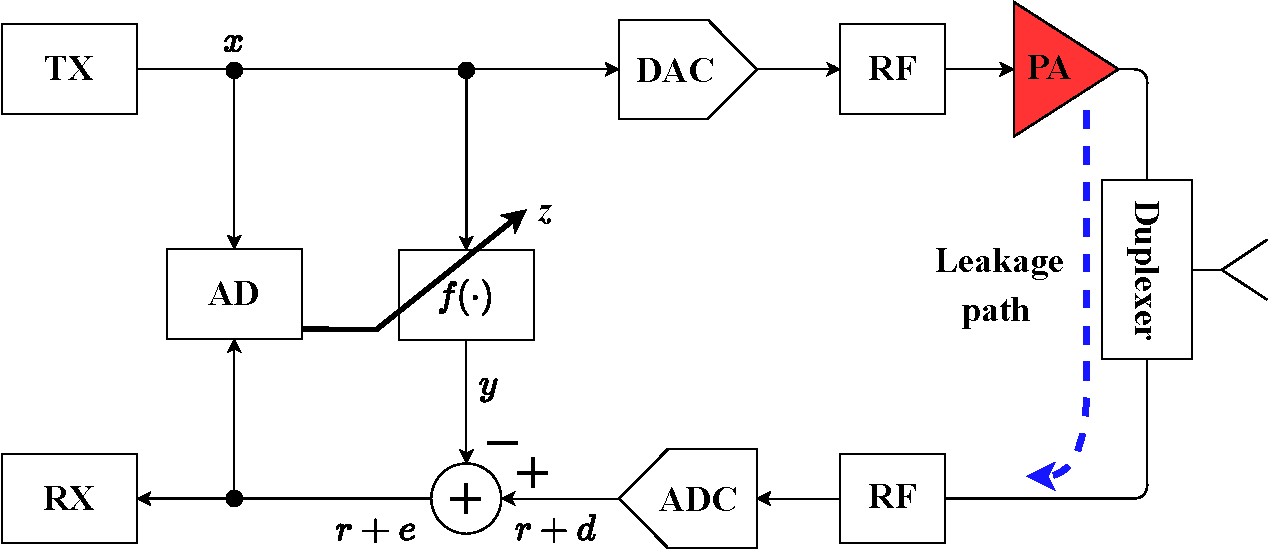
\includegraphics[width = 0.7\textwidth]{figures/ident_problem/ident_problem.pdf}}
\caption{Self-interference identification scheme.}
\label{ident_problem}
\end{figure}

\textbf{Self-interference cancellation issue.}
Conventional interference identification block scheme is shown in Fig.~\ref{ident_problem}. Transmitted signal samples $x_n$ are transformed to analog domain, then propagated through the nonlinear analog components, such as analog power amplifier (PA). Resulting nonlinear interference is distorted during propagation through the leakage path between transmitter and receiver. Thus, useful receiver signal is mixed with interference and transformed back to the digital samples $r_n+d_n$, where $r_n$ -- useful signal samples, $d_n$ -- interference samples. 

In order to get rid of parasitic interference $d_n$, adaptive signal processing block $\text{AD}$ in Fig.~\ref{ident_problem} adjusts parameters of the nonlinear block  $f = f(x_n, \bit{z})$, where \bit{z} -- nonlinear block parameters. Since useful signal $r_n$ has no correlation with interference, then adaptive processing block is supposed to minimize SI $d_n$. As a result, receiver samples are introduced by $r_n+e_n$, where $e_n=d_n-y_n=d_n-f(x_n, \bit{z})$.

SI minimization quality criteria is represented by Mean Square Error (MSE) \cite{behav_model}, since it is in fact algorithm error energy:
\begin{equation}
    \displaystyle\text{MSE}=\sum_{n=0}^{N-1}e_n^*e_n=\bit{e}^H\bit{e},
    \label{mse}
\end{equation}
where $\bit{e}=\bit{d}-\bit{y}$, $\bit{e}\in\mathbb{C}^{N\times 1}, \bit{d}\in\mathbb{C}^{N\times 1}, \bit{y}\in\mathbb{C}^{N\times 1}$, $N$ -- signal length, $(\cdot)^H$ -- hermitian conjugation operator.

\textbf{Interference model.}
Generally, behavioral modelling~\cite{behav_model} implies consideration of model which reflects physical processes of an appropriate phenomena. For instance, according to the Fig.~\ref{ident_problem} in SIC-task signal firstly distorted by nonlinearity in the transmitter path. After that, signal is affected by transmitter-receiver leakage path. Consequently, Hammerstein model~\cite{behav_model}, which is shown in Fig.~\ref{hammerstein_model} properly depicts behavior of parasitic interference. Note, that Hammerstein model is a simplification of Wiener-Hammerstein model~\cite{behav_model} for the case of memoryless non-linear effects.
\begin{figure}[h!]
\centerline{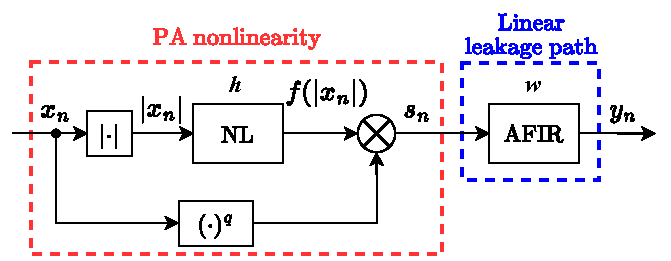
\includegraphics[width = 0.7\textwidth]{figures/hammerstein/hammerstein.pdf}}
\caption{Hammerstein model.}
\label{hammerstein_model}
\end{figure}
NL-block in Fig.~\ref{hammerstein_model} could be represented by various types of series, such as polynomials, trigonometric polynomials, splines etc. Nonetheless, in current work we have chosen 1~-~dimensional spline-based polynomial~\cite{lut_dpd} as a nonlinearity due to its low computational cost and easy hardware implementation. NL-block has parameters $\bit{h}\in\mathbb{C}^{P\times 1}$, $P$ -- polynomial order. AFIR-block shows adaptive FIR~\cite{haykin} with parameters $\bit{w}\in\mathbb{C}^{L\times 1}$, $L$ -- FIR order. Power $q$ in practice is chosen according to the intermodulation order. Since transmitter and receiver work in the same frequency band, then in current research $q=1$. Thus, model output sample could be derived as:
\begin{equation}
    y_n=\sum_{m=-D}^{D}w_m\sum_{k=0}^{P-1}h_k x_{n-m}NL(|x_{n-m}|),
    \label{hammerstein_output}
\end{equation}
where $L=2D+1$, $NL(\cdot)$ -- spline-based basis function~\cite{lut_dpd}, which is described in section \ref{mnm_for_hammer}.

% \textbf{SI Cancellation Algorithm}
% Current section is divided into the following parts. Firstly, Mixed Newton Method general approach and properties are given. Then, MNM application to the Hammerstein model is shown. 

\textbf{Mixed Newton general approach.}
Mixed Newton algorithm is a second-order method, designed for the training of complex-valued structures by minimization of MSE~\eqref{mse}. In addition, error vector $e_n=e_n(x_n, \bit{z})$~\eqref{mse} must be holomorphic with respect to the whole model parameters \bit{z}. In this case MNM has a property of repulsion from saddle points \cite{mixed_newton}.

Let operator $D_{\bit{z}}(\cdot)$ be a differentiation operator with model parameters vector $\bit{z}\in\mathbb{C}^{K\times 1}$, $K$-- number of whole model parameters:
\begin{equation}
    D_{\bit{z}}(\cdot)=\begin{pmatrix}
        \frac{\partial }{\partial z_0} &
        \frac{\partial }{\partial z_1} &
        \cdots &
        \frac{\partial }{\partial z_{K-1}}
    \end{pmatrix}
\end{equation}
Then, consider $D_{\bit{z}}J\in\mathbb{C}^{1\times K}$ as a scalar real-valued function $J\in\mathbb{R}$ derivative with respect to the whole model parameters. Thus, first-order differential of the function $J~=~J(\bit{z}, \bit{z}^*)$ could be derived as~\cite{complex_deriv}:
\begin{equation}
    dJ=D_{\bit{z}}Jd\bit{z}+D_{\bit{z}^*}Jd\bit{z}^*,
    \label{first_diff}
\end{equation}
where $D_{\bit{z}}J\in\mathbb{C}^{1\times K}$, $D_{\bit{z}^*}J\in\mathbb{C}^{1\times K}$, $d\bit{z}\in\mathbb{C}^{K\times 1}$, $d\bit{z}^*\in\mathbb{C}^{K\times 1}$.

Second-order derivative of scalar real-valued function $J$ is described as follows:

\begin{equation}
    D_{\bit{z}}(D_{\bit{z}}J)^T=H_{\bit{z}, \bit{z}}J\in\mathbb{C}^{K\times K}\text{-- Hessian matrix},
    \label{hessian_calc}
\end{equation}
where $(\cdot)^T$ -- transpose operator.

Using notations mentioned above, second-order differential of the function $J$ can be described in following way \cite{complex_deriv}:
\begin{equation}
    d^2J=\begin{pmatrix}
        d\bit{z}^T & d(\bit{z}^*)^T
    \end{pmatrix}
    \begin{pmatrix}
        H_{\bit{z}, \bit{z}}J & H_{\bit{z}^*, \bit{z}}J \\
        H_{\bit{z}, \bit{z}^*}J & H_{\bit{z}^*, \bit{z}^*}J
    \end{pmatrix}
    \begin{pmatrix}
        d\bit{z} \\ d\bit{z}^*
    \end{pmatrix}
\end{equation}
Since MNM algorithm uses only mixed hessian $H_{\bit{z}^*, \bit{z}}J$ for the model parameters training~\cite{mixed_newton}, then general view of its difference equation is as follows:
\begin{equation}
    \bit{z}_{k+1}=\bit{z}_k-\mu (H_{\bit{z}^*, \bit{z}} J)^{-1}(D_{\bit{z}^*}J)^T,
    \label{mixed_newton_eq}
\end{equation}
where $J$ -- MSE function, defined in \eqref{mse}.

Let us consider error vector $\bit{e}=\bit{e}(\bit{x}, \bit{z})\in\mathbb{C}^{N\times 1}$ as a holomorphic function with respect to \bit{z}. Then we can calculate MSE gradient and mixed hessian \eqref{mixed_newton_eq}. MSE gradient is derived as follows:
\begin{align}
    (D_{\bit{z}^*}J)^T=
    (D_{\bit{z}^*}(\bit{e}^H\bit{e}))^T=(D_{\bit{z}^*}(\bit{e}^T\bit{e}^*))^T= \nonumber \\=(\bit{e}^TD_{\bit{z}^*}\bit{e}^*)^T=(\bit{e}^T(D_{\bit{z}}\bit{e})^*)^T=(D_{\bit{z}}\bit{e})^H\bit{e}.
\end{align}
Since $\bit{e}=\bit{d}-\bit{y}(\bit{x}, \bit{z})$, where \bit{d} doesn`t depend on model parameters \bit{z}, then MSE gradient is as following:
\begin{equation}
    (D_{\bit{z}^*}J)^T=-(D_{\bit{z}}\bit{y})^H\bit{e},
    \label{grad}
\end{equation}
where $D_{\bit{z}}\bit{y}\in\mathbb{C}^{N\times K}$ -- model output Jacobian with respect to the whole model parameters.

In the same time, according to the notation \eqref{hessian_calc} and gradient expression \eqref{grad}, mixed hessian could be calculated in current way:
\begin{equation}
    H_{\bit{z}^*, \bit{z}}J=D_{\bit{z}}(D_{\bit{z}^*}J)^T=-D_{\bit{z}}((D_{\bit{z}}\bit{y})^H\bit{e}).
\end{equation}
Since \bit{y} is a holomorphic with respect to the model parameters, then mixed hessian is introduced by the following expression:
\begin{equation}
    H_{\bit{z}^*, \bit{z}}J=(D_{\bit{z}}\bit{y})^HD_{\bit{z}}\bit{y}.
    \label{mixed_hessian}
\end{equation}
Thus, considering expressions \eqref{grad}, \eqref{mixed_hessian} and \eqref{mixed_newton_eq}, Mixed Newton Method difference equation could represented as below:
\begin{equation}
    \bit{z}_{k+1}=\bit{z}_k-\mu ((D_{\bit{z}}\bit{y})^HD_{\bit{z}}\bit{y})^{-1}(D_{\bit{z}}\bit{y})^H\bit{e}.
    \label{mixed_newton_eq_jac}
\end{equation}
Thus, algorithm step requires calculation of an error \bit{e}, model output Jacobian with respect to the model parameters $D_{\bit{z}}\bit{y}$ and hessian inversion.

\textbf{Mixed Newton for Hammerstein model.} \label{mnm_for_hammer}
According to the difference equation \eqref{mixed_newton_eq_jac}, Mixed Newton requires calculation of model output Jacobian with respect to the whole model parameters \bit{z}. Hammerstein model is 2-layer model, which includes memoryless nonlinearity with parameters $\bit{h}\in\mathbb{C}^{P\times 1}$ and FIR with parameters $\bit{w}\in\mathbb{C}^{L\times 1}$. Consider Hammerstein model parameters vector and conjugated parameters vector as follows:
\begin{equation}
    \bit{z}=\begin{pmatrix}
        \bit{h} \\ \bit{w}
    \end{pmatrix},
    \bit{z}^*=\begin{pmatrix}
        \bit{h}^* \\ \bit{w}^*
    \end{pmatrix}
    \in\mathbb{C}^{(P+L)\times 1}.
\end{equation}
Then Hammerstein model output Jacobian with respect to the parameters is derived as below:
\begin{equation}
    D_{\bit{z}}\bit{y}=\begin{pmatrix}
        D_{\bit{h}}\bit{y} & D_{\bit{w}}\bit{y}
    \end{pmatrix}
    \in\mathbb{C}^{N\times(P+L)}.
    \label{jacobian_full}
\end{equation}
Thus we need to calculate model output vector derivative for the nonlinearity layer and FIR.

According to adaptive filtering theory \cite{haykin} FIR output could be derived through the state matrix \bit{U}:
\begin{equation}
    \bit{y}=\bit{U}\bit{w}, \bit{U}\in\mathbb{C}^{N\times L}.
    \label{fir_output}
\end{equation}
State matrix has following structure \cite{haykin}:
\begin{equation*}
    \bit{U}=
    \begin{pmatrix}
        s_{D} & \cdots & s_1 & s_0 & 0 & \cdots & 0 \\
        s_{D+1} & \cdots & s_2 & s_1 & s_0 & \cdots & 0 \\
        \vdots & & & \ddots & & & \vdots \\
        0 & \cdots & s_{N-1} & s_{N-2} & s_{N-3} & \cdots & s_{N-D-2} \\
        0 & \cdots & 0 & s_{N-1} & s_{N-2} & \cdots & s_{N-D-1} \\
    \end{pmatrix}.
    \label{fir_state_matrix}
\end{equation*}
Here $s_n$ -- FIR input sample in accordance with Fig.~\ref{hammerstein_model}. In correspondance with expression \eqref{hammerstein_output} FIR input sample could be shown as:
\begin{equation}
    s_n=\sum_{k=0}^{P-1}h_k x_{n}NL(|x_{n}|).
    \label{fir_input_sample}
\end{equation}
Since FIR state matrix doesn`t depend on FIR parameters \eqref{fir_input_sample}, then, according to \eqref{fir_output}, model output derivative with respect to the FIR parameters is:
\begin{equation}
    D_{\bit{w}}\bit{y}=D_{\bit{w}}(\bit{U}\bit{w})=\bit{U}.
    \label{jacobian_fir}
\end{equation}
Now, let us turn to the nonlinearity mathematical representation. Note, that spline polynomials operate as piecewise linear interpolation. In addition, this type of polynomial is efficient in terms of resources required for hardware implementation, that is why it has been chosen for behavioral modelling. 

Let us represent Hammerstein model output in matrix-vector multiplication manner through the spline-nonlinearity parameters vector. Consider FIR input vector as:
\begin{equation}
    \bit{s}=\bit{V}\bit{h}, \bit{V}\in\mathbb{C}^{N\times P}.
    \label{fir_input_vector}
\end{equation}
Nonlinearity state matrix \bit{V} for spline-based NL is shown below \cite{lut_dpd}:
\begin{equation*}
    \bit{V}=\begin{pmatrix}
        0 & 0 & \cdots & x_0(1-\Delta_0) & x_0\Delta_0 & \cdots & 0 \\
        0 & \cdots & x_1(1-\Delta_1) & x_1\Delta_1 & \cdots & 0 & 0 \\
        \vdots & & & \ddots & & & \vdots \\
        0 & 0 & \cdots & x_k(1-\Delta_k) & x_k\Delta_k & \cdots & 0 \\
        & & & \cdots & & &
    \end{pmatrix}.
\end{equation*}
Each row of state matrix \bit{V} include only 2 non-zero elements: $x_k(1-\Delta_k)$ and $x_k\Delta_k$, where $x_k$ - Hammerstein model input sample, $\Delta_k=||x_k|-\floor*{|x_k|}|$, where $\floor*{\cdot}$ -- floor operator. 

Current state matrix could be written through its columns:
\begin{equation}
    \bit{V}=\begin{pmatrix}
        \bit{v}_0 & \bit{v}_1 & \cdots & \bit{v}_{P-1}
    \end{pmatrix},
    \label{vand_matrix}
\end{equation}
then FIR input vector \eqref{fir_input_vector} is as below:
\begin{equation}
    \bit{s}=h_0\bit{v}_0+h_1\bit{v}_1+\cdots+h_{P-1}\bit{v}_{P-1}.
    \label{fir_input_vector_another}
\end{equation}
Thus, Hammerstein model output vector could be presented as:
\begin{equation}
    \bit{y}=\text{conv}_{w}(\bit{s}),
    \label{convolve_output}
\end{equation}
where $\text{conv}_{w}(\cdot)$ -- 1-dimensional linear convolution operator. Using convolution linearity property, equations \eqref{fir_input_vector_another} and \eqref{convolve_output} we obtain Hammerstein model output through matrix-vactor multiplication:
\begin{multline}
    \bit{y}=\text{conv}_{w}(h_0\bit{v}_0+\cdots+h_{P-1}\bit{v}_{P-1})
    =h_0\text{conv}_{w}(\bit{v}_0)+\cdots+h_{P-1}\text{conv}_{w}(\bit{v}_{P-1})= \\
    =\begin{pmatrix}
        \text{conv}_{w}(\bit{v}_0) & \cdots & \text{conv}_{w}(\bit{v}_{P-1})
    \end{pmatrix}\bit{h}\equiv\bit{V}_f\bit{h}.
    \label{nonlin_output}
\end{multline}
Therefore, Hammerstein model output vector is derived through the product of nonlinearity state matrix, filtered across columns, and nonlinearity parameters vector. Note, that matrix $\bit{V}_f$ doesn`t depend on spline polynomial parameters \bit{h}.

As a result, using equation \eqref{nonlin_output}, model output derivative with respect to nonlinearity parameters could be written as:
\begin{equation}
    D_{\bit{h}}\bit{y}=D_{\bit{h}}(\bit{V}_f\bit{h})=\bit{V}_f.
    \label{jacobian_nonlin}
\end{equation}
Finally, using expressions for model output Jacobians \eqref{jacobian_full}, \eqref{jacobian_fir}, \eqref{jacobian_nonlin}, Mixed Newton difference equation \eqref{mixed_newton_eq_jac} could be rewritten as:
\begin{equation}
    \bit{z}_{k+1}=\bit{z}_k+\mu\begin{pmatrix}
        \bit{V}_f^H\bit{V}_f & \bit{V}_f^H\bit{U} \\
        \bit{U}^H\bit{V}_f & \bit{U}^H\bit{U}
    \end{pmatrix}^{-1}\begin{pmatrix}
        \bit{V}_f^H \\
        \bit{U}^H
    \end{pmatrix}\bit{e}.
    \label{mixed_newton_eq_jac_hammer}
\end{equation}
Note, that algorithm \eqref{mixed_newton_eq_jac_hammer} can be modified by additional step size $\mu$ tuning. In our computations parameter $\mu$ is adjusted in accordance with the solution of the one-dimensional optimization problem every training epoch.

Also, notice that Gradient Descent approach for Hammerstein model is represented by the following expression:
\begin{equation}
    \bit{z}_{k+1}=\bit{z}_k+\mu (D_{\bit{z}^*}J)^T=
    \bit{z}_k+\mu\begin{pmatrix}
        \bit{V}_f^H \\
        \bit{U}^H
    \end{pmatrix}\bit{e}.
    \label{gd_eq_jac_hammer}
\end{equation}


%In this section, we describe simulation setup, present experimental results for Mixed Newton Method (MNM) and compare them with Block Gradient Descent (BGD) and Stochastic Gradient Descent (SGD) in terms of convergence speed and final performance. 

Computational complexity of the MNM step~\eqref{mixed_newton_eq_jac_hammer} is determined by matrices $\bit{U}$~\eqref{jacobian_fir}, $\bit{V}_f$~\eqref{jacobian_nonlin} calculation, gradient $D_{\bit{z}^*}J$~\eqref{gd_eq_jac_hammer}, inverse Hessian-gradient product, calculation and, the most important, mixed Hessian $H_{\bit{z}^*, \bit{z}}J$~\eqref{mixed_hessian} calculation and inversion.

Signal sample propagation through the spline-based nonlinearity~\eqref{fir_input_sample} is estimated as $\mathcal{O}(1)$ float-point operations (FLOPs), then whole signal $\bit{x}\in\mathbb{C}^{N\times 1}$ propagation through nonlinearity and, as a result, matrices $\bit{U}$ and $\bit{V}$ calculation require $\mathcal{O}(N)$ calculations. Matrix $\bit{V}$~\eqref{vand_matrix} filtering could be evaluated as $\mathcal{O}(PLN)$. 

Gradient and Hessian calculation requires $\mathcal{O}((P+L)N)$ and $\mathcal{O}((P+L)^2N)$ operations respectively. Inverse Hessian-gradient product complexity is $\mathcal{O}((P+L)^2)$. Hessian inversion is the most complex operation among mentioned. Since mixed Hessian for holomorphic funcitons is hermitian matrix, then matrix inversion could be implemented by means of eigenvalue decomposition (EVD), its complexity is estimated as $\mathcal{O}((P+L)^3)$~\cite{matrix_comput}.

According to aforementioned, whole algorithm step complexity is evaluated as:
\begin{align}
    \chi_{MNM}=&\mathcal{O}(N)+\mathcal{O}(PLN)+\mathcal{O}((P+L)N)+\mathcal{O}((P+L)^2N)+\mathcal{O}((P+L)^2)+ \nonumber \\
    &+\mathcal{O}((P+L)^3)=\mathcal{O}((P+L)^3+(P+~L)^2N).
    \label{complexity_mnm}
\end{align}
Thus, Hessian calculation and inversion are the most difficult in terms of FLOPs number.

It can be seen, that gradient descent complexity is sufficiently lower, since it requires only matrices $\bit{U}$, $\bit{V}_f$ and gradient calculation:
\begin{equation}
    \chi_{grad}=\mathcal{O}(N)+\mathcal{O}(PLN)+\mathcal{O}((P+L)N)=\mathcal{O}(PLN+(P+L)N).
    \label{complexity_grad}
\end{equation}
Nevertheless, gradient descent steps in real application might be made much faster comparing to MNM steps. As a result, gradient-based methods require sufficiently more steps. Consequently, number of FLOPs for both approaches may probably differ insignificantly.

%\textbf{Experimental setup}
\textbf{Numerical Results.} The transmitter data is provided by QAM-modulated OFDM signal with 60 MHz pass-band bandwidth. The sample rate is 484 MHz. The whole data consists of $\sim$80000 samples, with 50\% is used for training and the rest samples used for testing. 

Testbench is shown in fig.~\ref{install}. Digital transmitter data is sent to the signal generator, where it is transformed to the analog domain and moved to the 1.7 GHz carrier frequency.
\begin{figure}[h!]
    \centering
    \captionsetup{justification=centering}
    \centerline{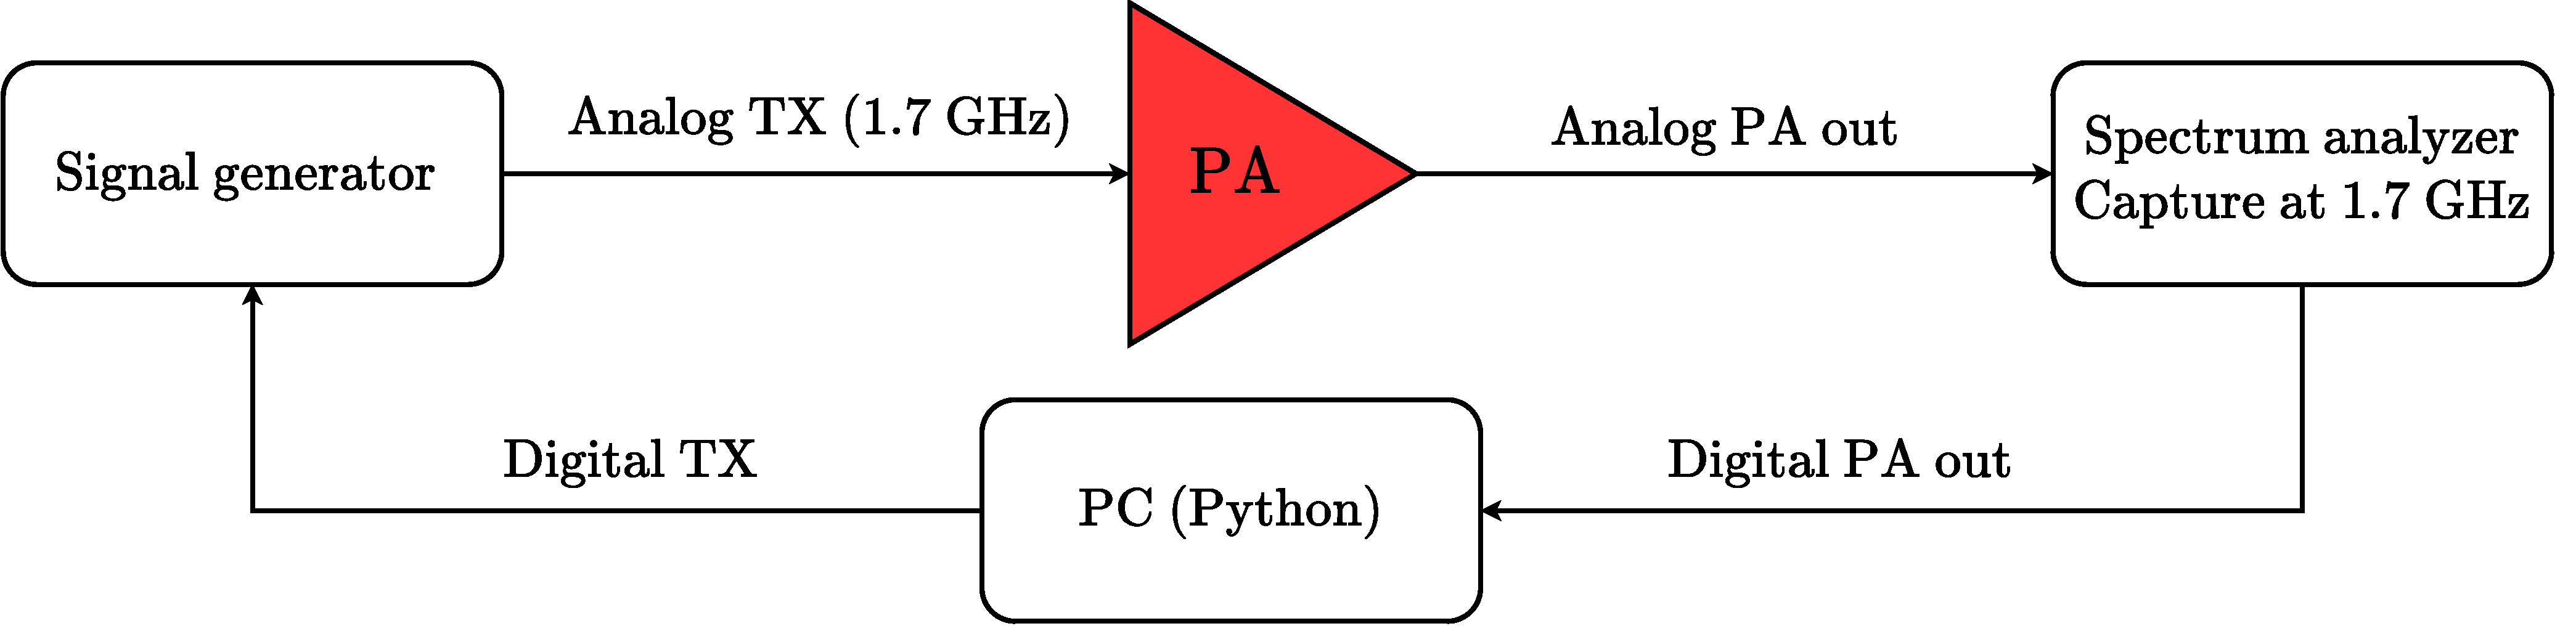
\includegraphics[width = 0.8\textwidth]{figures/install/install.pdf}}
    \caption{Testbench scheme for signal nonlinear distortion generation}
    \label{install}
\end{figure}
Then, it propagated through the PA with average output power 20 dBm and captured by means of spectrum analyzer at 1.7 GHz. Captured signal is further sent back to the PC. Leakage path is simulated by digital FIR order 51. Captured PA out is propagated through the generated filter. FIR output signal is considered as the self-interference.

Note, that in real application interference is mixed with useful receiver signal as in Fig.~\ref{ident_problem}. In this case adaptive correction module suppresses only self-interference, due to useful signal might have no correlation with transmitter signal~\cite{haykin}. Therefore, in our simulations we don`t take into account useful RX-signal and consider only SI as the receiver path.

For SIC experiments we have chosen Hammerstein model~(Fig.~\ref{hammerstein_model}) with $L=45$ taps adaptive FIR, 1-dimensional linear-spline polynomial order $P=8$. In exponentiation branch $q=1$.

All provided results were made on NVIDIA Tesla V100 GPU with 16 GB RAM.

\textbf{Cancellation Performance and Convergence Speed.}
Mixed Newton and BGD are applied to whole training data. In other words, matrices $V_f$ and $U$ in equations \eqref{mixed_newton_eq_jac_hammer}, \eqref{gd_eq_jac_hammer} are calculated for $\sim$40000 samples. 

On the other hand, in case of SGD whole training set is divided into the non-overlapping blocks, which are packed into the batches. Each batch consist of 50~blocks of 200~samples. Thus each epoch model trains on 4~batches. Gradients are calculated for each block in batch and averaged. Batch size and block size were chosen experimentally in terms if the highest performance.

Also, notice that in BGD and MNM model parameters are updated once per epoch, whereas in SGD parameters -- once per batch.

In following simulations NMSE is tracked every epoch on train and test data, which is shown in fig.~\ref{lc_mnm_bgd},~\ref{lc_mnm_sgd}.

\begin{figure}[h!]
    \centering
    \captionsetup{justification=centering}
    \centerline{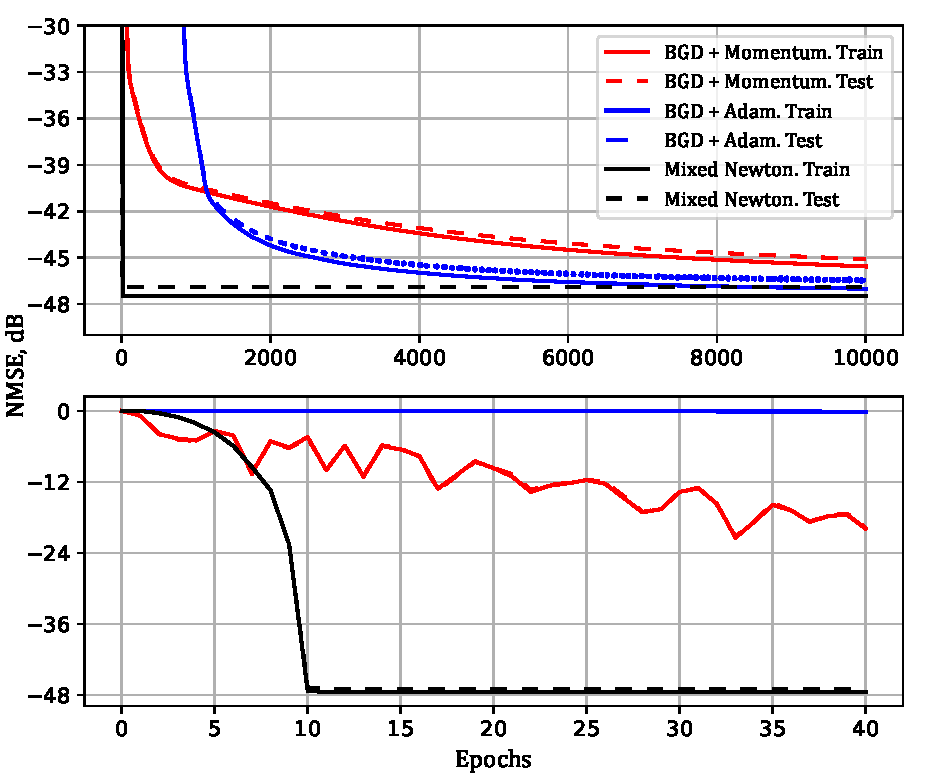
\includegraphics[width = 0.7\textwidth]{figures/mnm_bgd/mnm_bgd.pdf}}
    \caption{BGD with Momentum, BGD with Adam and MNM learning curves on train and test data sets}
    \label{lc_mnm_bgd}
\end{figure}

Convergence speed comparison of Block Gradient Descent with Momentum and Adam optimizers, and Mixed Newton are shown in Fig~\ref{lc_mnm_bgd}. MNM requires approximately 30 epochs to achieve final performance, whereas BGD with both optimizers require $\sim10000$ epochs to acquire the same NMSE.

Fig.~\ref{lc_mnm_sgd} represents learning curves obtained for SGD with Momentum and Adam optimizers and Mixed Newton. It can be seen that SGD also requires approximately $10000$ epochs to achieve performance obtained by MNM.
\begin{figure}[h!]
    \centering
    \captionsetup{justification=centering}
    \centerline{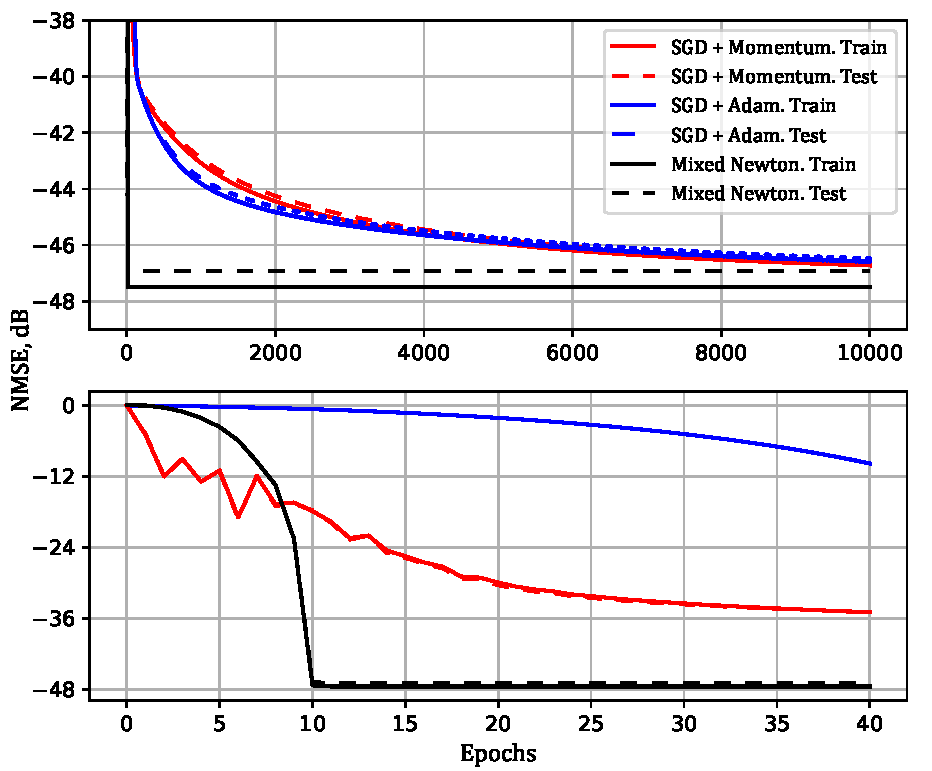
\includegraphics[width = 0.7\textwidth]{figures/mnm_sgd/mnm_sgd.pdf}}
    \caption{SGD with Momentum, SGD with Adam and MNM learning curves on train and test data sets}
    \label{lc_mnm_sgd}
\end{figure}

Note, that optimizers parameters and learning rate for gradient descent where chosen in the way to achieve the best final performance and the highest convergence speed.

Power spectral densities (PSD) of the initial and suppressed by different methods interference are shown in Fig.~\ref{psd}. PSD figures are built on test data set.
\begin{figure}[h!]
    \centering
    \captionsetup{justification=centering}
    \centerline{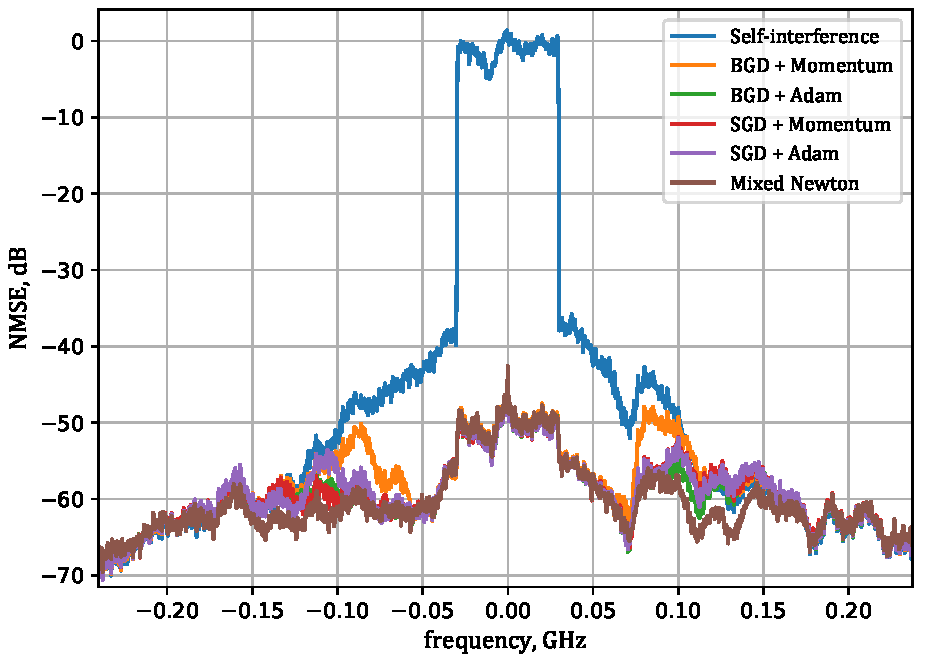
\includegraphics[width = 0.7\textwidth]{figures/psd/psd.pdf}}
    \caption{PSD of initial and suppressed interference}
    \label{psd}
\end{figure}

Table~\ref{table_of_results} shows remarkable convergence speed increase of Mixed Newton method comparing to the common gradient methods used in the interference suppression tasks. MNM requires only 30 epochs to achieve comparable performance. Although, provided second order method requires sufficiently less optimization steps, the steps in current simulation~$\sim5$ times longer. Nevertheless, total time required for training is significantly decreased.
\begin{table}[h!]
\centering
    \caption{Performance and convergence speed comparison}
    \begin{tabular}{|l|c|c|c|c|c|}
    \hline
    \textbf{Algorithm} &
      \textbf{\begin{tabular}[c]{@{}c@{}}BGD\\ Moment.\end{tabular}} &
      \textbf{\begin{tabular}[c]{@{}c@{}}BGD\\ Adam\end{tabular}} &
      \textbf{\begin{tabular}[c]{@{}c@{}}SGD \\ Moment.\end{tabular}} &
      \textbf{\begin{tabular}[c]{@{}c@{}}SGD \\ Adam\end{tabular}} &
      \textbf{MNM} \\ \hline
    \textbf{\begin{tabular}[c]{@{}l@{}}Epoch\\ number\end{tabular}} &
      {\color[HTML]{000000} 10000} &
      {\color[HTML]{000000} 10000} &
      {\color[HTML]{000000} 10000} &
      10000 &
      30 \\ \hline
    \textbf{\begin{tabular}[c]{@{}l@{}}Time per\\ epoch, $10^{-2}$ s\end{tabular}} &
      {\color[HTML]{000000} 3.8} &
      {\color[HTML]{000000} 4.0} &
      {\color[HTML]{000000} 3.7} &
      4.1 &
      21 \\ \hline
    \textbf{\begin{tabular}[c]{@{}l@{}}Total elapsed\\ tims, s\end{tabular}} &
      {\color[HTML]{000000} 380} &
      {\color[HTML]{000000} 403} &
      {\color[HTML]{000000} 386} &
      412 &
      6.2 \\ \hline
        \multirow{2}{*}{\textbf{NMSE, dB}} &
        \multirow{2}{*}{-45.1} &
        \multirow{2}{*}{-46.7} &
        \multirow{2}{*}{-46.6} &
        \multirow{2}{*}{-46.5} &
        \multirow{2}{*}{-46.9} \\ 
        & & & & & \\ \hline 
    \end{tabular}
    \label{table_of_results}
\end{table}

According to calculations provided in theoretical part, MNM step complexity~\eqref{complexity_mnm} is high comparing to the gradient-based algorithms~\eqref{complexity_grad}. Nonetheless number of steps, required for convergence is significantly lower for Mixed Newton (table~\ref{table_of_results}). Thus, MNM is remarkably suitable for offline model performance estimation. Also, Mixed Newton could be exploited for online models training, since in real application it requires mixed Hessian accumulation and, as a result, makes significantly lower training steps comparing to gradient-based methods.

\textbf{Conclusion.}
In current paper, we provided a novel method of SI cancellation. The method is strictly derived for Hammerstein model case using matrix differentiation approach. Although, Mixed Newton requires~$\sim5$~times longer calculation step, total training duration is sufficiently decreased to 30 epochs, instead of 10000 required for conventional first-order optimization methods, to achieve the same interference cancellation level $46.9$ dB. 

Future work may consider an application of proposed second-order algorithm for training of non-linear interference models, which are introduced by Complex-Valued Neural Networks (CVNNs). Since Mixed Newton implies inverse matrix calculation, it has high memory consumption. Therefore current algorithm, in its original view, could be implemented only for low-complexity NNs and doesn`t scale to the high-complexity models. Thus, crucial research direction is introduced by modification of MNM in order to minimize Hessian inversion overhead, which, for instance, could be represented by various inverse matrix estimation techniques.

\AtNextBibliography{\footnotesize}
\printbibliography

\end{document}
